\documentclass[12pt,]{krantz}
\usepackage{lmodern}
\usepackage{amssymb,amsmath}
\usepackage{ifxetex,ifluatex}
\usepackage{fixltx2e} % provides \textsubscript
\ifnum 0\ifxetex 1\fi\ifluatex 1\fi=0 % if pdftex
  \usepackage[T1]{fontenc}
  \usepackage[utf8]{inputenc}
\else % if luatex or xelatex
  \ifxetex
    \usepackage{mathspec}
  \else
    \usepackage{fontspec}
  \fi
  \defaultfontfeatures{Ligatures=TeX,Scale=MatchLowercase}
\fi
% use upquote if available, for straight quotes in verbatim environments
\IfFileExists{upquote.sty}{\usepackage{upquote}}{}
% use microtype if available
\IfFileExists{microtype.sty}{%
\usepackage[]{microtype}
\UseMicrotypeSet[protrusion]{basicmath} % disable protrusion for tt fonts
}{}
\PassOptionsToPackage{hyphens}{url} % url is loaded by hyperref
\usepackage[unicode=true]{hyperref}
\PassOptionsToPackage{usenames,dvipsnames}{color} % color is loaded by hyperref
\hypersetup{
            pdftitle={Series de Tiempo en R},
            pdfauthor={Synergy Vision},
            colorlinks=true,
            linkcolor=Maroon,
            citecolor=Blue,
            urlcolor=Blue,
            breaklinks=true}
\urlstyle{same}  % don't use monospace font for urls
\usepackage{natbib}
\bibliographystyle{apalike}
\usepackage{color}
\usepackage{fancyvrb}
\newcommand{\VerbBar}{|}
\newcommand{\VERB}{\Verb[commandchars=\\\{\}]}
\DefineVerbatimEnvironment{Highlighting}{Verbatim}{commandchars=\\\{\}}
% Add ',fontsize=\small' for more characters per line
\usepackage{framed}
\definecolor{shadecolor}{RGB}{248,248,248}
\newenvironment{Shaded}{\begin{snugshade}}{\end{snugshade}}
\newcommand{\KeywordTok}[1]{\textcolor[rgb]{0.13,0.29,0.53}{\textbf{#1}}}
\newcommand{\DataTypeTok}[1]{\textcolor[rgb]{0.13,0.29,0.53}{#1}}
\newcommand{\DecValTok}[1]{\textcolor[rgb]{0.00,0.00,0.81}{#1}}
\newcommand{\BaseNTok}[1]{\textcolor[rgb]{0.00,0.00,0.81}{#1}}
\newcommand{\FloatTok}[1]{\textcolor[rgb]{0.00,0.00,0.81}{#1}}
\newcommand{\ConstantTok}[1]{\textcolor[rgb]{0.00,0.00,0.00}{#1}}
\newcommand{\CharTok}[1]{\textcolor[rgb]{0.31,0.60,0.02}{#1}}
\newcommand{\SpecialCharTok}[1]{\textcolor[rgb]{0.00,0.00,0.00}{#1}}
\newcommand{\StringTok}[1]{\textcolor[rgb]{0.31,0.60,0.02}{#1}}
\newcommand{\VerbatimStringTok}[1]{\textcolor[rgb]{0.31,0.60,0.02}{#1}}
\newcommand{\SpecialStringTok}[1]{\textcolor[rgb]{0.31,0.60,0.02}{#1}}
\newcommand{\ImportTok}[1]{#1}
\newcommand{\CommentTok}[1]{\textcolor[rgb]{0.56,0.35,0.01}{\textit{#1}}}
\newcommand{\DocumentationTok}[1]{\textcolor[rgb]{0.56,0.35,0.01}{\textbf{\textit{#1}}}}
\newcommand{\AnnotationTok}[1]{\textcolor[rgb]{0.56,0.35,0.01}{\textbf{\textit{#1}}}}
\newcommand{\CommentVarTok}[1]{\textcolor[rgb]{0.56,0.35,0.01}{\textbf{\textit{#1}}}}
\newcommand{\OtherTok}[1]{\textcolor[rgb]{0.56,0.35,0.01}{#1}}
\newcommand{\FunctionTok}[1]{\textcolor[rgb]{0.00,0.00,0.00}{#1}}
\newcommand{\VariableTok}[1]{\textcolor[rgb]{0.00,0.00,0.00}{#1}}
\newcommand{\ControlFlowTok}[1]{\textcolor[rgb]{0.13,0.29,0.53}{\textbf{#1}}}
\newcommand{\OperatorTok}[1]{\textcolor[rgb]{0.81,0.36,0.00}{\textbf{#1}}}
\newcommand{\BuiltInTok}[1]{#1}
\newcommand{\ExtensionTok}[1]{#1}
\newcommand{\PreprocessorTok}[1]{\textcolor[rgb]{0.56,0.35,0.01}{\textit{#1}}}
\newcommand{\AttributeTok}[1]{\textcolor[rgb]{0.77,0.63,0.00}{#1}}
\newcommand{\RegionMarkerTok}[1]{#1}
\newcommand{\InformationTok}[1]{\textcolor[rgb]{0.56,0.35,0.01}{\textbf{\textit{#1}}}}
\newcommand{\WarningTok}[1]{\textcolor[rgb]{0.56,0.35,0.01}{\textbf{\textit{#1}}}}
\newcommand{\AlertTok}[1]{\textcolor[rgb]{0.94,0.16,0.16}{#1}}
\newcommand{\ErrorTok}[1]{\textcolor[rgb]{0.64,0.00,0.00}{\textbf{#1}}}
\newcommand{\NormalTok}[1]{#1}
\usepackage{longtable,booktabs}
% Fix footnotes in tables (requires footnote package)
\IfFileExists{footnote.sty}{\usepackage{footnote}\makesavenoteenv{long table}}{}
\usepackage{graphicx,grffile}
\makeatletter
\def\maxwidth{\ifdim\Gin@nat@width>\linewidth\linewidth\else\Gin@nat@width\fi}
\def\maxheight{\ifdim\Gin@nat@height>\textheight\textheight\else\Gin@nat@height\fi}
\makeatother
% Scale images if necessary, so that they will not overflow the page
% margins by default, and it is still possible to overwrite the defaults
% using explicit options in \includegraphics[width, height, ...]{}
\setkeys{Gin}{width=\maxwidth,height=\maxheight,keepaspectratio}
\IfFileExists{parskip.sty}{%
\usepackage{parskip}
}{% else
\setlength{\parindent}{0pt}
\setlength{\parskip}{6pt plus 2pt minus 1pt}
}
\setlength{\emergencystretch}{3em}  % prevent overfull lines
\providecommand{\tightlist}{%
  \setlength{\itemsep}{0pt}\setlength{\parskip}{0pt}}
\setcounter{secnumdepth}{5}
% Redefines (sub)paragraphs to behave more like sections
\ifx\paragraph\undefined\else
\let\oldparagraph\paragraph
\renewcommand{\paragraph}[1]{\oldparagraph{#1}\mbox{}}
\fi
\ifx\subparagraph\undefined\else
\let\oldsubparagraph\subparagraph
\renewcommand{\subparagraph}[1]{\oldsubparagraph{#1}\mbox{}}
\fi

% set default figure placement to htbp
\makeatletter
\def\fps@figure{htbp}
\makeatother

\usepackage[T1]{fontenc}
\usepackage[utf8]{inputenc} % recommended encoding
\usepackage[spanish]{babel}
\usepackage{booktabs}
\usepackage{longtable}
\usepackage[bf,singlelinecheck=off]{caption}

%\setmainfont[UprightFeatures={SmallCapsFont=AlegreyaSC-Regular}]{Alegreya}

\usepackage{framed,color}
\definecolor{shadecolor}{RGB}{248,248,248}

\renewcommand{\textfraction}{0.05}
\renewcommand{\topfraction}{0.8}
\renewcommand{\bottomfraction}{0.8}
\renewcommand{\floatpagefraction}{0.75}

\renewenvironment{quote}{\begin{VF}}{\end{VF}}
\let\oldhref\href
\renewcommand{\href}[2]{#2\footnote{\url{#1}}}

\ifxetex
  \usepackage{letltxmacro}
  \setlength{\XeTeXLinkMargin}{1pt}
  \LetLtxMacro\SavedIncludeGraphics\includegraphics
  \def\includegraphics#1#{% #1 catches optional stuff (star/opt. arg.)
    \IncludeGraphicsAux{#1}%
  }%
  \newcommand*{\IncludeGraphicsAux}[2]{%
    \XeTeXLinkBox{%
      \SavedIncludeGraphics#1{#2}%
    }%
  }%
\fi

\makeatletter
\newenvironment{kframe}{%
\medskip{}
\setlength{\fboxsep}{.8em}
 \def\at@end@of@kframe{}%
 \ifinner\ifhmode%
  \def\at@end@of@kframe{\end{minipage}}%
  \begin{minipage}{\columnwidth}%
 \fi\fi%
 \def\FrameCommand##1{\hskip\@totalleftmargin \hskip-\fboxsep
 \colorbox{shadecolor}{##1}\hskip-\fboxsep
     % There is no \\@totalrightmargin, so:
     \hskip-\linewidth \hskip-\@totalleftmargin \hskip\columnwidth}%
 \MakeFramed {\advance\hsize-\width
   \@totalleftmargin\z@ \linewidth\hsize
   \@setminipage}}%
 {\par\unskip\endMakeFramed%
 \at@end@of@kframe}
\makeatother

\renewenvironment{Shaded}{\begin{kframe}}{\end{kframe}}

\newenvironment{rmdblock}[1]
  {
  \begin{itemize}
  \renewcommand{\labelitemi}{
    \raisebox{-.7\height}[0pt][0pt]{
      {\setkeys{Gin}{width=3em,keepaspectratio}\includegraphics{images/#1}}
    }
  }
  \setlength{\fboxsep}{1em}
  \begin{kframe}
  \item
  }
  {
  \end{kframe}
  \end{itemize}
  }
\newenvironment{rmdnote}
  {\begin{rmdblock}{note}}
  {\end{rmdblock}}
\newenvironment{rmdcaution}
  {\begin{rmdblock}{caution}}
  {\end{rmdblock}}
\newenvironment{rmdimportant}
  {\begin{rmdblock}{important}}
  {\end{rmdblock}}
\newenvironment{rmdtip}
  {\begin{rmdblock}{tip}}
  {\end{rmdblock}}
\newenvironment{rmdwarning}
  {\begin{rmdblock}{warning}}
  {\end{rmdblock}}

\usepackage{makeidx}
\makeindex

\urlstyle{tt}

\usepackage{amsthm}
\makeatletter
\def\thm@space@setup{%
  \thm@preskip=8pt plus 2pt minus 4pt
  \thm@postskip=\thm@preskip
}
\makeatother

\frontmatter

\title{Series de Tiempo en R}
\providecommand{\subtitle}[1]{}
\subtitle{Ciencia de los Datos Financieros}
\author{Synergy Vision}
\date{2018-03-20}

\usepackage{amsthm}
\newtheorem{theorem}{Teorema}[chapter]
\newtheorem{lemma}{Lema}[chapter]
\theoremstyle{definition}
\newtheorem{definition}{Definición}[chapter]
\newtheorem{corollary}{Corolario}[chapter]
\newtheorem{proposition}{Proposición}[chapter]
\theoremstyle{definition}
\newtheorem{example}{Ejemplo}[chapter]
\theoremstyle{definition}
\newtheorem{exercise}{Ejercicio}[chapter]
\theoremstyle{remark}
\newtheorem*{remark}{Nota}
\newtheorem*{solution}{Solución}
\let\BeginKnitrBlock\begin \let\EndKnitrBlock\end
\begin{document}
\maketitle

%\cleardoublepage\newpage\thispagestyle{empty}\null
%\cleardoublepage\newpage\thispagestyle{empty}\null
%\cleardoublepage\newpage
\thispagestyle{empty}
\begin{center}
%\includegraphics{images/dedication.pdf}
\end{center}

\setlength{\abovedisplayskip}{-5pt}
\setlength{\abovedisplayshortskip}{-5pt}

{
\hypersetup{linkcolor=black}
\setcounter{tocdepth}{2}
\tableofcontents
}
\listoftables
\listoffigures
\chapter*{Prefacio}\label{prefacio}



\includegraphics{images/by-nc-sa.png}\\
La versión en línea de este libro se comparte bajo la licencia
\href{http://creativecommons.org/licenses/by-nc-sa/4.0/}{Creative
Commons Attribution-NonCommercial-ShareAlike 4.0 International License}.

\section*{¿Por qué leer este libro?}\label{por-que-leer-este-libro}


\section*{Estructura del libro}\label{estructura-del-libro}


\section*{Información sobre los programas y
convenciones}\label{informacion-sobre-los-programas-y-convenciones}
\addcontentsline{toc}{section}{Información sobre los programas y
convenciones}

Este libro es posible gracias a una gran cantidad de desarrolladores que
contribuyen en la construcción de herramientas para generar documentos
enriquecidos e interactivos. En particular al autor de los paquetes
Yihui Xie xie2015.

\section*{Prácticas interactivas con
R}\label{practicas-interactivas-con-r}


Vamos a utilizar el paquete
\href{https://github.com/datacamp/tutorial}{Datacamp Tutorial} que
utiliza la librería en JavaScript
\href{https://github.com/datacamp/datacamp-light}{Datacamp Light} para
crear ejercicios y prácticas con \texttt{R}. De esta forma el libro es
completamente interactivo y con prácticas incluidas. De esta forma
estamos creando una experiencia única de aprendizaje en línea.

eyJsYW5ndWFnZSI6InIiLCJwcmVfZXhlcmNpc2VfY29kZSI6ImIgPC0gNSIsInNhbXBsZSI6IiMgQ3JlYSB1bmEgdmFyaWFibGUgYSwgaWd1YWwgYSA1XG5cblxuIyBNdWVzdHJhIGVsIHZhbG9yIGRlIGEiLCJzb2x1dGlvbiI6IiMgQ3JlYSB1bmEgdmFyaWFibGUgYSwgaWd1YWwgYSA1XG5hIDwtIDVcblxuIyBNdWVzdHJhIGVsIHZhbG9yIGRlIGFcbmEiLCJzY3QiOiJ0ZXN0X29iamVjdChcImFcIilcbnRlc3Rfb3V0cHV0X2NvbnRhaW5zKFwiYVwiLCBpbmNvcnJlY3RfbXNnID0gXCJBc2VnJnVhY3V0ZTtyYXRlIGRlIG1vc3RyYXIgZWwgdmFsb3IgZGUgYGFgLlwiKVxuc3VjY2Vzc19tc2coXCJFeGNlbGVudGUhXCIpIn0=

\section*{Agradecimientos}\label{agradecimientos}


\BeginKnitrBlock{flushright}
Synergy Vision, Caracas, Venezuela
\EndKnitrBlock{flushright}

\chapter*{Acerca del Autor}\label{acerca-del-autor}


Este material es un esfuerzo de equipo en Synergy Vision,
(\url{http://synergy.vision/nosotros/}).

El propósito de este material es ofrecer una experiencia de aprendizaje
distinta y enfocada en el estudiante. El propósito es que realmente
aprenda y practique con mucha intensidad. La idea es cambiar el modelo
de clases magistrales y ofrecer una experiencia más centrada en el
estudiante y menos centrado en el profesor. Para los temas más técnicos
y avanzados es necesario trabajar de la mano con el estudiante y
asistirlo en el proceso de aprendizaje con prácticas guiadas, material
en línea e interactivo, videos, evaluación contínua de brechas y
entendimiento, entre otros, para procurar el dominio de la materia.

Nuestro foco es la Ciencia de los Datos Financieros y para ello se
desarrollará material sobre: \textbf{Probabilidad y Estadística
Matemática en R}, \textbf{Programación Científica en R},
\textbf{Mercados}, \textbf{Inversiones y Trading}, \textbf{Datos y
Modelos Financieros en R}, \textbf{Renta Fija}, \textbf{Inmunización de
Carteras de Renta Fija}, \textbf{Teoría de Riesgo en R},
\textbf{Finanzas Cuantitativas}, \textbf{Ingeniería Financiera},
\textbf{Procesos Estocásticos en R}, \textbf{Series de Tiempo en R},
\textbf{Ciencia de los Datos}, \textbf{Ciencia de los Datos
Financieros}, \textbf{Simulación en R}, \textbf{Desarrollo de
Aplicaciones Interactivas en R}, \textbf{Minería de Datos},
\textbf{Aprendizaje Estadístico}, \textbf{Estadística Multivariante},
\textbf{Riesgo de Crédito}, \textbf{Riesgo de Liquidez}, \textbf{Riesgo
de Mercado}, \textbf{Riesgo Operacional}, \textbf{Riesgo de Cambio},
\textbf{Análisis Técnico}, \textbf{Inversión Visual}, \textbf{Finanzas},
\textbf{Finanzas Corporativas}, \textbf{Valoración}, \textbf{Teoría de
Portafolio}, entre otros.

Nuestra cuenta de Twitter es (\url{https://twitter.com/bysynergyvision})
y nuestros repositorios están en GitHub
(\url{https://github.com/synergyvision}).

\textbf{Somos Científicos de Datos Financieros}

\chapter{Introducción}\label{introduccion}

Las series de tiempo ya han desempeñado un papel importante en las
primeras ciencias naturales. La astronomía babilónica utilizó series de
tiempo de las posiciones relativas de estrellas y planetas para predecir
eventos astronómicos. Las observaciones de los movimientos de los
planetas formaron la base de las leyes que Johannes Kepler descubrió. El
análisis de las series de tiempo ayuda a detectar las regularidades en
las observaciones de una variable y a derivar ``leyes'' de ellas, y/o
explotar toda la información incluida en esta variable para predecir
mejor los desarrollos futuros. La idea metodológica básica detrás de
estos procedimientos, que también eran válidos para los babilonios, es
que es posible descomponer series de tiempos en un número finito de
componentes independientes pero no directamente observables que se
desarrollan regularmente y que por lo tanto pueden ser calculados de
antemano. Para este procedimiento es necesario que existan diferentes
factores independientes que incidan en la variable. A mediados del siglo
XIX, este enfoque metodológico de la astronomía fue asumido por los
economistas Charles Babbage y William Stanley Jevons. La descomposición
en componentes no observados que dependen de diferentes factores
causales, como suele emplearse en el análisis clásico de series de
tiempo, fue desarrollada por Warren M. Persons (1919). Distinguía cuatro
componentes diferentes:

\begin{itemize}
\item
  Desarrollo a largo plazo, tendencia,
\item
  Componente cíclico con períodos de más de un año, el ciclo económico,
\item
  Componente que contiene los altibajos dentro de un año, el ciclo
  estacional, y
\item
  Componente que contiene todos los movimientos que no pertenecen ni a
  la tendencia ni al ciclo económico ni al componente estacional, el
  residual.
\end{itemize}

Suponiendo que los diferentes factores no observables son
independientes, su recubrimiento aditivo genera las series de tiempo
que, sin embargo, sólo podemos observar en su conjunto. Para obtener
información sobre el proceso de generación de datos, tenemos que hacer
suposiciones sobre sus componentes no observados. El análisis clásico de
series de tiempo supone que los componentes sistemáticos, es decir, la
tendencia, el ciclo económico y el ciclo estacional, no están
influenciados por perturbaciones estocásticas y, por lo tanto, pueden
representarse mediante funciones determinísticas del tiempo. El impacto
estocástico se limita a los residuos, que, por otra parte, no contienen
movimientos sistemáticos. Por lo tanto, se modela como una serie de
variables aleatorias independientes o no correlacionadas con esperanza
cero y varianza constante, es decir, como un proceso aleatorio puro.

Este enfoque cambió desde la presentación de los trabajos de George E.
P. Box and Gwilym M. Jenkins, ``Time Series Analysis: Forecasting and
Control'', en los años 70 del siglo pasado. Se abandonaron los
procedimientos puramente descriptivos del análisis clásico de series de
tiempo y, en su lugar, se han utilizado los resultados y métodos de la
teoría de la probabilidad y las estadísticas matemáticas. Desde ese
entonces, el análisis de series ha tenido un desarrollo creciente. Se
han presentado una gran variedad de libros sobre este tópico, cada uno
de ellos influenciado principalmente por la orientación de las series
que se discuten en sus contenidos. Una gran parte de la literatura está
dirigida a exponer los aspectos teóricos alrededor de las series de
tiempo, siendo en muchos casos, rigurosamente desarrollados y descritos,
sin embargo poco de ellos presentan implementaciones de las técnicas
estudiadas y su compresión en ejemplos reales lo que a veces puede
dificultar su comprensión en especial para aquellos que no posean una
apropiada formación matemática.

Los primeros intentos de estudiar el comportamiento de las series de
tiempo financieras fueron realizados por profesionales financieros y
periodistas en lugar de por académicos. De hecho, esto parece haberse
convertido en una tradición de larga data, ya que, incluso hoy en día,
gran parte de la investigación y el desarrollo empíricos todavía se
originan en la propia industria financiera. Esto puede explicarse por el
carácter práctico de los problemas, la necesidad de datos especializados
y las posibles ventajas de dicho análisis. El primer y más conocido
ejemplo de la investigación publicada sobre series de tiempo financieras
es el legendario Charles Dow, como se expresa en sus editoriales en el
Wall Street Times entre 1900 y 1902. Estos escritos formaron la base de
la ``teoría del Dow'' e influyeron en lo que más tarde se conoció como
análisis técnico y carisma. Aunque Dow no coleccionó y publicó sus
editoriales por separado, esto fue hecho póstumamente por su seguidor
Samuel Nelson (Nelson, 1902). Las ideas originales de Dow fueron
posteriormente interpretadas y ampliadas por Hamilton (1922) y Rhea
(1932). Estas ideas gozaron de cierto reconocimiento entre los
académicos de la época: por ejemplo, Hamilton fue elegido miembro de la
Royal Statistical Society.

Aunque Dow y sus seguidores discutieron muchas de las ideas que
encontramos en el análisis moderno de finanzas y series de tiempo,
incluyendo estacionalidad, eficiencia del mercado, correlación entre
rendimiento de activos e índices, diversificación e imprevisibilidad, no
hicieron ningún esfuerzo serio para adoptar métodos estadísticos
formales. La mayor parte del análisis empírico consistió en la
interpretación minuciosa de gráficos detallados de las medias bursátiles
sectoriales, formando así los famosos índices Dow-Jones. Se argumentó
que estos índices descuentan toda la información necesaria y
proporcionan el mejor pronóstico de eventos futuros. Una idea
fundamental, muy relevante para la teoría de los ciclos de Stanley
Jevons y la metodología de descomposición de tendencias de la ``curva
Harvard A-B-C'' de Warren Persons, fue que las variaciones de precios
del mercado consistían en tres movimientos primarios: diarios, a medio y
largo plazo.

La investigación empírica más temprana que utiliza métodos estadísticos
formales se remonta a los documentos de Working (1934), Cowles
(1933,1944) y Cowles and Jones (1937). El trabajo centró la atención en
una característica previamente señalada de los precios de las materias
primas y las acciones: que se asemejan a la acumulación de cambios
puramente aleatorios. Alfred Cowles 3rd, analista financiero
cuantitativamente entrenado y fundador de Econometric Society and the
Cowles Foundation, investigó la habilidad de los analistas de mercado y
servicios financieros para predecir los futuros cambios de precios,
encontrando que había pocas pruebas de que pudieran hacerlo. Cowles y
Jones reportaron evidencia de correlación positiva entre sucesivas
variaciones de precios, pero, como posteriormente Cowles (1960) comentó,
esto fue probablemente debido a que tomaron promedios mensuales de
precios diarios o semanales antes de computar los cambios: un fenómeno
de ``correlación espuria'', analizado por Working (1960).

La previsibilidad de los cambios de precios se ha convertido desde
entonces en un tema importante de la investigación financiera, pero,
sorprendentemente, poco más se publicó hasta el estudio de Kendall
(1953), en el que encontró que los cambios semanales en una amplia
variedad de precios financieros no podían predecirse ni a partir de los
cambios pasados en las series ni a partir de los cambios pasados en
otras series de precios. Este parece haber sido el primer informe
explícito de esta propiedad de los precios financieros a menudo citada,
aunque la investigación sobre la previsibilidad de los precios sólo se
vio impulsada por la publicación de los documentos de Roberts (1959) y
Osborne (1959). El primero presenta un argumento en gran medida
heurístico sobre por qué las sucesivas variaciones de precios deben ser
independientes, mientras que el segundo desarrolla la proposición de que
no se trata de cambios absolutos de precios, sino de cambios
logarítmicos de precios independientes entre sí. Con la suposición
auxiliar de que las propias modificaciones se distribuyen normalmente,
esto implica que los precios se generan como movimiento Browniano.

El análisis de series de tiempo desempeña un papel importante en el
análisis requerido para el pronóstico de eventos futuros. Existen varias
formas o métodos de calcular cual va a ser la tendencia del
comportamiento del proceso en estudio.

Un \textbf{pronóstico} es una predicción de algún evento o eventos
futuros. Como sugirió Neils Bohr, hacer buenas predicciones no siempre
es fácil. Los pronósticos famosamente ``malos'' incluyen lo siguiente
del libro \emph{``Malas Predicciones''}:

\begin{itemize}
\item
  ``La población es de tamaño constante y se mantendrá hasta el fin de
  la humanidad.'' La Enciclopedia, 1756.
\item
  ``1930 será un espléndido año de empleo.'' Departamento de Trabajo de
  los EE. UU., pronóstico de Año Nuevo en 1929, justo antes de que el
  mercado se desplomara el 29 de octubre.
\item
  ``Las computadoras se multiplican a un ritmo rápido. Para el cambio de
  siglo habrá 220,000 en los EE. UU.'' Wall Street Journal, 1966.
\end{itemize}

Algunos ejemplos donde se puede utilizar y hacer precciones con series
de tiempo:

\begin{enumerate}
\def\labelenumi{\arabic{enumi})}
\item
  \textbf{Dirección de Operaciones}. Las organizaciones empresariales
  utilizan habitualmente las previsiones de ventas de productos o la
  demanda de servicios para programar la producción, controlar los
  inventarios, gestionar la cadena de suministro, determinar las
  necesidades de personal y planificar la capacidad. Las previsiones
  también pueden utilizarse para determinar la combinación de productos
  o servicios que deben ofrecerse y las ubicaciones en las que deben
  fabricarse los productos.
\item
  \textbf{Marketing}. La previsión es importante en muchas decisiones de
  marketing. Las previsiones de respuesta de las ventas a los gastos
  publicitarios, las nuevas romociones o los cambios en las políticas de
  precios permiten a las empresas evaluar su eficacia, determinar si se
  están alcanzando los objetivos y realizar ajustes.
\item
  \textbf{Finanzas y Gestión de Riesgos}. Los inversores en activos
  financieros están interesados en pronosticar los rendimientos de sus
  inversiones. Estos activos incluyen, pero no se limitan a acciones,
  bonos y materias primas; otras decisiones de inversión se pueden tomar
  en relación con las previsiones de tasas de interés, opciones y tipos
  de cambio. La gestión del riesgo financiero requiere previsiones de la
  volatilidad de la rentabilidad de los activos para que se puedan
  evaluar y asegurar los riesgos asociados a las carteras de inversión,
  y para que los derivados financieros puedan cotizarse adecuadamente.
\item
  \textbf{Economía}. Los gobiernos, las instituciones financieras y las
  organizaciones de política requieren pronósticos de las principales
  variables económicas, como el producto interno bruto, el crecimiento
  demográfico, el desempleo, las tasas de interés, la inflación, el
  crecimiento del empleo, la producción y el consumo. Estas previsiones
  son parte integrante de la orientación de la política monetaria y
  fiscal, así como de los planes y decisiones presupuestarias adoptadas
  por los gobiernos. También son fundamentales en las decisiones de
  planificación estratégica tomadas por organizaciones empresariales e
  instituciones financieras.
\item
  \textbf{Control de Procesos Industriales}. Las previsiones de los
  valores futuros de las características de calidad crítica de un
  proceso de producción pueden ayudar a determinar cuándo deben
  cambiarse las variables controlables importantes del proceso, o si el
  proceso debe detenerse y revisarse. Los esquemas de retroalimentación
  y control feedforward son ampliamente utilizados en el monitoreo y
  ajuste de procesos industriales, y las predicciones de la producción
  del proceso son una parte integral de estos esquemas.
\item
  \textbf{Demografía}. Las previsiones de población por país y región se
  realizan de manera rutinaria, a menudo estratificadas por variables
  como el género, la edad y la raza. Los demógrafos también pronostican
  nacimientos, muertes y patrones migratorios de las poblaciones. Los
  gobiernos utilizan estas previsiones para planificar políticas y
  acciones de servicio social, como el gasto en atención médica,
  programas de jubilación y programas de lucha contra la pobreza. Muchas
  empresas utilizan pronósticos de poblaciones por grupos de edad para
  hacer planes estratégicos en relación con el desarrollo de nuevas
  líneas de productos o tipos de servicios que será ofrecido.
\end{enumerate}

\section{Conceptos básicos}\label{conceptos-basicos}

Una serie tiempo es una secuencia de observaciones, medidos en
determinados momentos del tiempo, ordenados cronológicamente y,
espaciados entre sí de manera uniforme, así los datos usualmente son
dependientes entre sí. El principal objetivo de una serie de tiempo es
su análisis para hacer pronóstico. Formalmente se tiene la siguiente
definición.

\BeginKnitrBlock{definition}
\protect\hypertarget{def:defi-serie-tiempo}{}{\label{def:defi-serie-tiempo}
}Una \textbf{serie de tiempo} es un conjunto de observaciones \(x_t\),
cada una registrada a un tiempo específico \(t\).
\EndKnitrBlock{definition}

\BeginKnitrBlock{definition}
\protect\hypertarget{def:defi-modelo-serie-tiempo}{}{\label{def:defi-modelo-serie-tiempo}
}Un \textbf{modelo de series de tiempo} para los datos observados
\(\{x_t\}\) es una especificación de una distribución conjunta (o
posiblemente solo de medias y covarianzas) de una sucesión de variables
aleatorias \(\{X_t\}\) de las cuales \(\{x_t\}\) es una realización.
\EndKnitrBlock{definition}

A continuación presentaremos una serie de ejemplos que demuestran la
utilidad y lo cotidiano de las series de tiempo, también se mostrarán
los códigos en R para cargar los archivos de datos y graficar las
respectivas series de tiempo.

\section{Ejemplos}\label{ejemplos}

\BeginKnitrBlock{example}
\protect\hypertarget{exm:ejem-beneficios-acciones}{}{\label{exm:ejem-beneficios-acciones}
}\textbf{Beneficios de acciones.} Beneficios por acción trimestrales
para la compañía Johnson \& Johnson. Se tienen 84 trimestres iniciando
el primer trimestre de 1960 hasta el último trimestre de 1980. Los
métodos para analizar tales datos se verán en el Tema 3 usando técnicas
de regresión. El archivo es \emph{``jj.txt''}.

Los comandos en R para cargar el archivo y graficar la serie de tiempo
son los siguientes:
\EndKnitrBlock{example}

\begin{Shaded}
\begin{Highlighting}[]
\NormalTok{jj=}\KeywordTok{ts}\NormalTok{(}\KeywordTok{scan}\NormalTok{(}\StringTok{"data/jj.txt"}\NormalTok{),}\DataTypeTok{start=}\DecValTok{1960}\NormalTok{,}\DataTypeTok{freq=}\DecValTok{4}\NormalTok{) }
\KeywordTok{plot}\NormalTok{(jj, }\DataTypeTok{type=}\StringTok{"l"}\NormalTok{,}\DataTypeTok{ylab=}\StringTok{"Beneficios por acción trimestrales"}\NormalTok{)}
\end{Highlighting}
\end{Shaded}

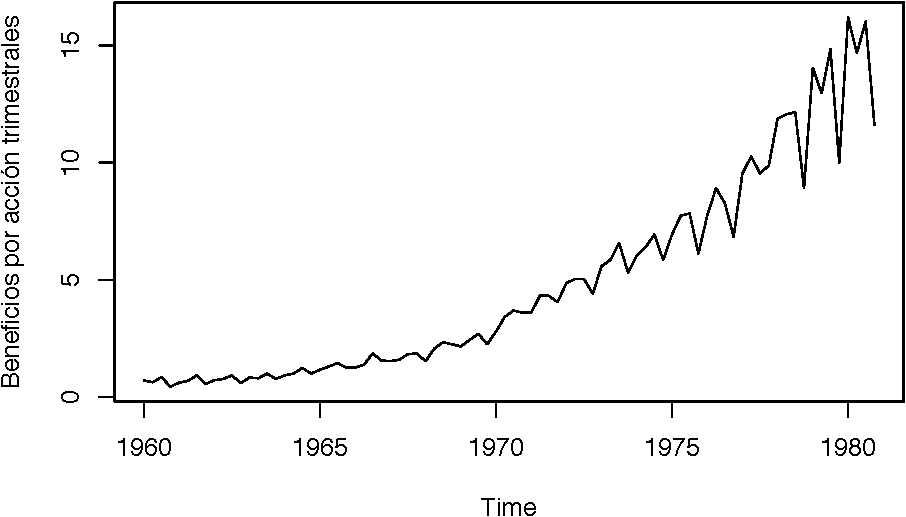
\includegraphics{Serie-de-Tiempo-en-R_files/figure-latex/unnamed-chunk-8-1.pdf}

\BeginKnitrBlock{example}
\protect\hypertarget{exm:reservas-internacionales}{}{\label{exm:reservas-internacionales}
}El archivo \emph{``ReservasInternacionales.xlsx''}, contiene el
registro mensual de Reservas Internacionales Venezolanas en millones de
dólares (\$), iniciando en el mes de enero de 1996 hasta el mes de
diciembre de 2017
\EndKnitrBlock{example}

\begin{Shaded}
\begin{Highlighting}[]
\CommentTok{#library(readxl)}
\NormalTok{reservas <-}\StringTok{ }\KeywordTok{read_excel}\NormalTok{(}\StringTok{"data/ReservasInternacionales.xlsx"}\NormalTok{)}
\NormalTok{reservas=}\KeywordTok{ts}\NormalTok{(reservas,}\DataTypeTok{start =} \DecValTok{1996}\NormalTok{,}\DataTypeTok{frequency =} \DecValTok{12}\NormalTok{)}
\KeywordTok{plot.ts}\NormalTok{(reservas[,}\DecValTok{2}\NormalTok{], }\DataTypeTok{xlab=}\StringTok{"Año"}\NormalTok{,}\DataTypeTok{ylab=}\StringTok{"Monto"}\NormalTok{,}
        \DataTypeTok{main=}\StringTok{"Reservas Internacionales de Venezuela (millones $)"}\NormalTok{)}
\end{Highlighting}
\end{Shaded}

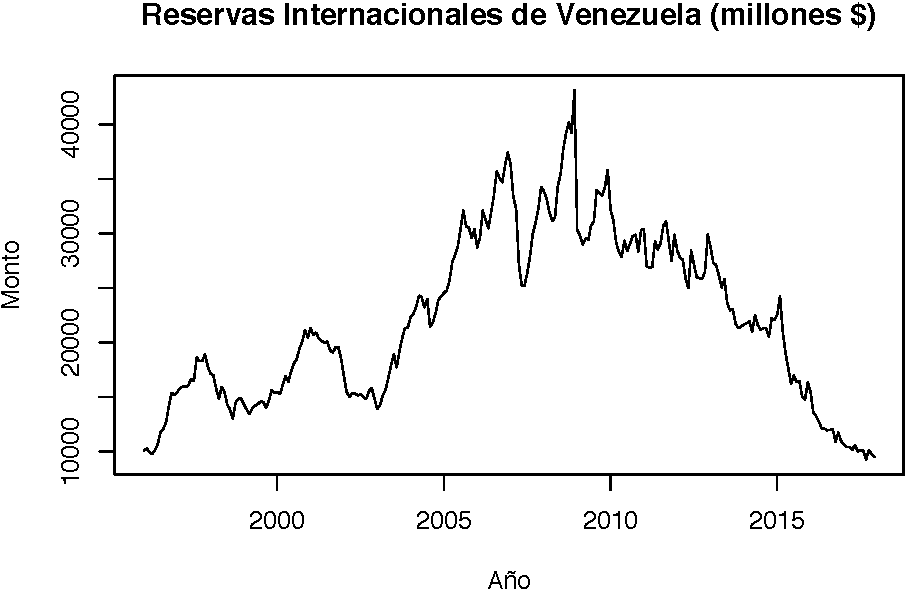
\includegraphics{Serie-de-Tiempo-en-R_files/figure-latex/unnamed-chunk-9-1.pdf}

\BeginKnitrBlock{example}
\protect\hypertarget{exm:precio-petroleo}{}{\label{exm:precio-petroleo} }El
archivo \emph{``PreciosPetroleoVzla.xlsx''} contiene el precio promedio
mensual de venta para el petróleo venezolano (en dólares) desde enero
2006 hasta noviembre 2017
\EndKnitrBlock{example}

\begin{Shaded}
\begin{Highlighting}[]
\CommentTok{# library(readxl)}
\NormalTok{petroleo <-}\StringTok{ }\KeywordTok{read_excel}\NormalTok{(}\StringTok{"data/PreciosPetroleoVzla.xlsx"}\NormalTok{)}
\NormalTok{petroleo=}\KeywordTok{ts}\NormalTok{(petroleo,}\DataTypeTok{start =} \DecValTok{2006}\NormalTok{,}\DataTypeTok{frequency =} \DecValTok{12}\NormalTok{)}
\KeywordTok{plot.ts}\NormalTok{(petroleo[,}\DecValTok{2}\NormalTok{], }\DataTypeTok{xlab=}\StringTok{"Año"}\NormalTok{,}\DataTypeTok{ylab=}\StringTok{"Monto"}\NormalTok{,}
        \DataTypeTok{main=}\StringTok{"Precio promedio del petróleo venezolano (en dolares $)"}\NormalTok{)}
\end{Highlighting}
\end{Shaded}

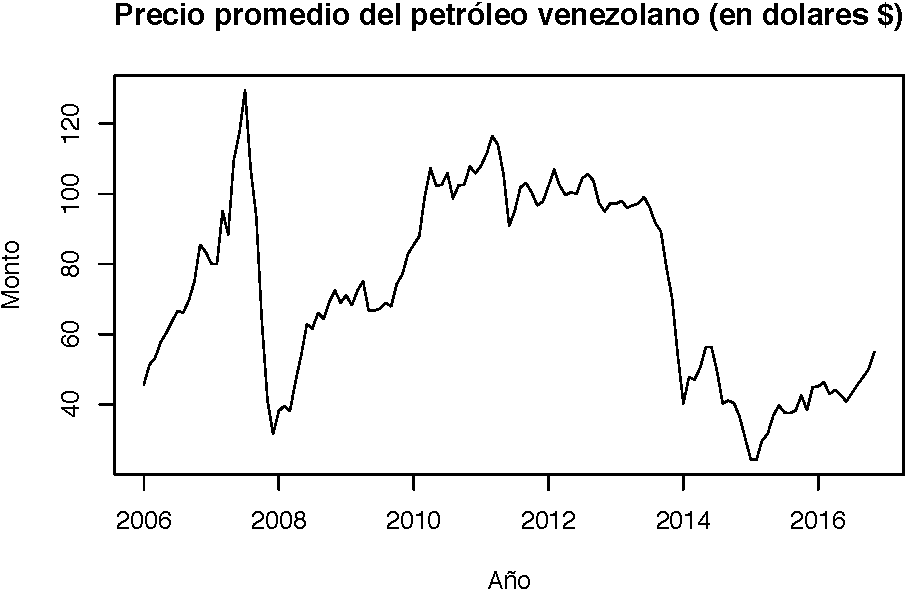
\includegraphics{Serie-de-Tiempo-en-R_files/figure-latex/unnamed-chunk-10-1.pdf}

\BeginKnitrBlock{example}
\protect\hypertarget{exm:indice-dow-jones}{}{\label{exm:indice-dow-jones}
}El archivo \emph{``IndiceDowJones.xlsx''} contiene los valores
histórico del índice Dow-Jones desde enero de 1930 hasta octubre de
2017. En el archivo podems notar que desde enero de 1930 hasta diciembre
de 1994, los registros son el promedio semanal, a partir de enero de
1995, los registros son diarios. La primera columa es la fecha, la
segunda columna es el valor de apertura, la tercera columna el valor
máximo, la cuarta el valor mínimo, la quinta el último valor del índice
o valor de cierre y la sexta columna es el volumen de acciones.
\EndKnitrBlock{example}

\begin{Shaded}
\begin{Highlighting}[]
\NormalTok{DJ=}\KeywordTok{read_excel}\NormalTok{(}\StringTok{"data/IndiceDowJones.xlsx"}\NormalTok{)}
\NormalTok{DJ=}\KeywordTok{ts}\NormalTok{(DJ)}
\KeywordTok{plot.ts}\NormalTok{(DJ[,}\OperatorTok{-}\DecValTok{1}\NormalTok{], }\DataTypeTok{xlab=}\StringTok{"Días"}\NormalTok{,}
        \DataTypeTok{main=}\StringTok{"Índice Dow-Jones desde enero 1930 hasta octubre 2017"}\NormalTok{)}
\end{Highlighting}
\end{Shaded}

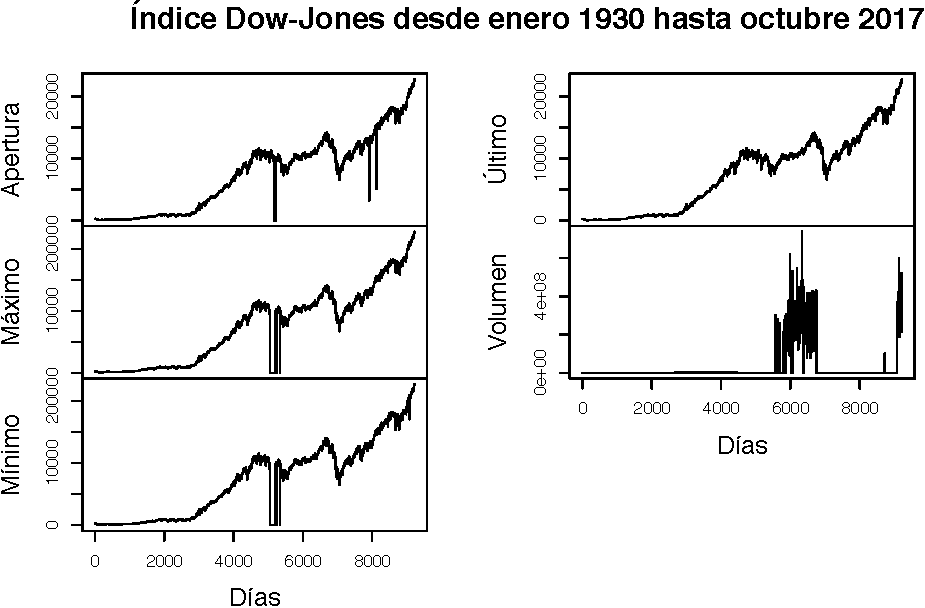
\includegraphics{Serie-de-Tiempo-en-R_files/figure-latex/unnamed-chunk-11-1.pdf}

\BeginKnitrBlock{example}
\protect\hypertarget{exm:Bolsa-Valores-New-York}{}{\label{exm:Bolsa-Valores-New-York}
}La figura siguiente muestra los porcentajes de cambio diario de la
Bolsa de Valores de New York desde el 2 de febrero de 1984 hasta el 31
de diciembre de 1991. Como se ve hay una caída fuerte, esta ocurrió el
19 de octubre de 1987 en \(t=938\). El archivo de datos es
\emph{``nyse.txt''}.
\EndKnitrBlock{example}

\begin{Shaded}
\begin{Highlighting}[]
\NormalTok{NYSE=}\KeywordTok{ts}\NormalTok{(}\KeywordTok{scan}\NormalTok{(}\StringTok{"data/nyse.txt"}\NormalTok{))}
\KeywordTok{plot}\NormalTok{(NYSE,}\DataTypeTok{xlab=}\StringTok{"Tiempo"}\NormalTok{,}\DataTypeTok{ylab=}\StringTok{"Porcentaje de cambio, NYSE"}\NormalTok{)}
\end{Highlighting}
\end{Shaded}

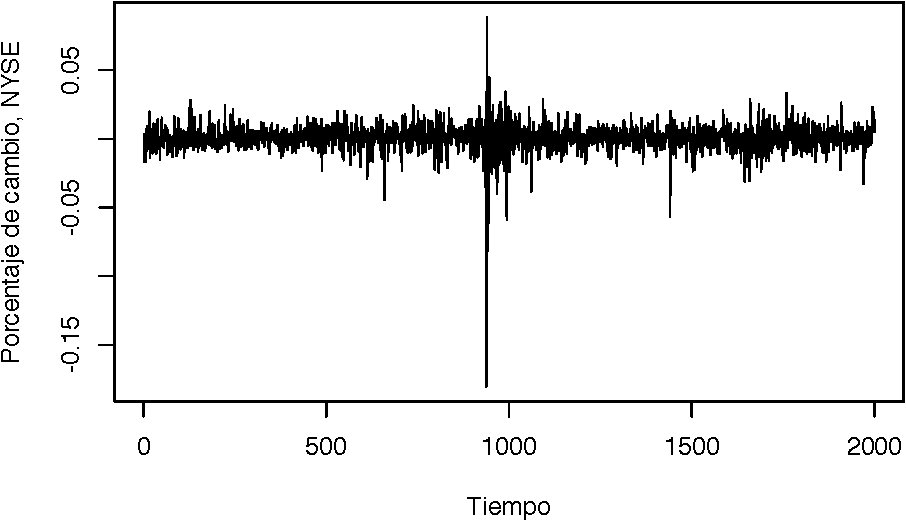
\includegraphics{Serie-de-Tiempo-en-R_files/figure-latex/unnamed-chunk-12-1.pdf}

\subsection{Clasificación de las series de
tiempo}\label{clasificacion-de-las-series-de-tiempo}

Como se ha mostrado en los ejemplos anteriores, hay una amplia variedad
de series de tiempo que pueden clasificarse en varias categorías desde
varios puntos de vista.

\begin{itemize}
\item
  \textbf{Series de tiempo continuas y discretas}. Los datos registrados
  continuamente, por ejemplo, por un dispositivo analógico, se denominan
  series de tiempo continuas. Por otra parte, los datos observados en
  ciertos intervalos de tiempo, como la presión atmosférica medida cada
  hora, se denominan series de tiempo discretas. Existen dos tipos de
  series de tiempo discretas: una en la que las observaciones de los
  datos se realizan a intervalos de igual espaciamiento y otra en la que
  las observaciones de los datos se realizan a intervalos de
  espaciamiento desigual. Aunque las series de tiempo mostradas en los
  ejemplos anteriores están conectadas continuamente por líneas sólidas,
  todas ellas son series de tiempo discretas. A partir de ahora en este
  libro, consideramos sólo discretas series de tiempo grabadas a
  intervalos igualmente espaciados, porque las series de tiempo que
  analizamos en ordenadores digitales son generalmente series de tiempo
  discretas.
\item
  \textbf{Series de tiempo univariadas y multivariadas}. Las series de
  tiempo que consisten en una sola observación en cada punto temporal,
  como se muestran en los ejemplos 1.1, 1.2, 1.3 y 1.5, se denominan
  series de tiempo univariadas. Por otra parte, las series de tiempo que
  se obtienen grabando simultáneamente dos o más fenómenos como los
  ilustrados en el ejemplo 1.4 se denominan series de tiempo
  multivariadas. Sin embargo, puede ser difícil distinguir entre series
  de tiempo univariadas y multivariadas desde su naturaleza; más bien,
  la distinción se hace desde el punto de vista del analista y por
  varios otros factores, como la restricción de la medición y los
  conocimientos empíricos o teóricos sobre el tema. Desde el punto de
  vista del modelado estadístico, la selección de variables en sí misma
  es un problema importante en el análisis de series de tiempo.
\item
  \textbf{Series de tiempo estacionarias y no estacionarias}. Una serie
  de tiempo es un registro de un fenómeno que varía irregularmente con
  el tiempo. En el análisis de series de tiempo, las series de tiempo de
  variación irregular se expresan generalmente mediante modelos
  estocásticos. En algunos casos, un fenómeno aleatorio puede ser
  considerado como la realización de un modelo estocástico con una
  estructura de variación temporal. Estas series de tiempo se denominan
  series de tiempo estacinarias. El ejemplo 1.5 es un ejemplo típico de
  una serie de tiempo estacionaria. Por otra parte, si la estructura
  estocástica de una serie de tiempo cambia con el tiempo, se denomina
  serie de tiempo no estacionaria. Como ejemplos típicos de series de
  tiempo no estacionarias, considere la serie en los ejemplos 1.1 a 1.4
  . Se puede observar que los valores medios cambian a lo largo del
  tiempo.
\item
  \textbf{Series de tiempo gaussianas y no gaussianas}. Cuando una
  distribución de una serie de tiempo sigue una distribución normal, la
  serie de tiempo se denomina serie de tiempo gaussiana; de lo
  contrario, se denomina serie de tiempo no gausiana. La mayoría de los
  modelos considerados en este libro son modelos gaussianos, asumiendo
  que las series de tiempo siguen distribuciones gaussianas. Al igual
  que en el caso del ejemplo 1.3, el patrón de las series de tiempo es a
  veces asimétrico, de modo que la distribución marginal no puede
  considerarse gaussiana. Incluso en tal situación, podemos obtener una
  serie de tiempo gaussiana aproximada mediante una transformación de
  datos apropiada.
\item
  \textbf{Series de tiempo lineales y no lineales}. Una serie de tiempo
  expresable como la salida de un modelo lineal se denomina serie de
  tiempo lineal. Por el contrario, la salida de un modelo no lineal se
  denomina serie de tiempo no lineal.
\item
  \textbf{Datos faltantes y valores atípicos}. En el modelado de series
  de tiempo de problemas del mundo real, a veces necesitamos tratar con
  observaciones faltante y valores atípicos. Algunos valores de las
  series de tiempo que no se han registrado por algunas razones se
  denominan observaciones que faltan en las series de tiempo. Los
  valores atípicos (observaciones exteriores) pueden ocurrir debido al
  comportamiento extraordinario del objeto, mal funcionamiento del
  dispositivo de observación o errores en el registro. En los datos de
  los ejemplos 1.4 y 1.5 se pueden observar datos atípicos. En el
  ejemplo 1.4 podemos notar caídas en los índices del DowJones y en el
  ejemplo 1.4 podemos notar una fuerte caída en el porcentaje de cambio
  de diario ocurrido el 19 de octubre de 1987.
\end{itemize}

\section{Componentes de una serie de
tiempo}\label{componentes-de-una-serie-de-tiempo}

El análisis clásico de las series de tiempo se basa en la suposición de
que los valores que toma la variable de observación es la consecuencia
de tres componentes, cuya actuación conjunta da como resultado los
valores medidos, estos componentes son:

\begin{enumerate}
\def\labelenumi{\arabic{enumi})}
\item
  \textbf{Componente de tendencia}. Se puede definir como un cambio a
  largo plazo que se produce en la relación al nivel medio, o el cambio
  a largo plazo de la media. La tendencia se identifica con un
  movimiento suave de la serie a largo plazo.
\item
  \textbf{Componente estacional}. Muchas series de tiempo presentan
  cierta periodicidad o dicho de otro modo, variación de cierto período
  (semestral, mensual, etc.). Por ejemplo las Ventas al Detalle en
  Puerto Rico aumentan por los meses de noviembre y diciembre por las
  festividades navideñas. Estos efectos son fáciles de entender y se
  pueden medir explícitamente o incluso se pueden eliminar de la serie
  de datos, a este proceso se le llama desestacionalización de la serie.
\item
  \textbf{Componente aleatoria}. Esta componente no responde a ningún
  patrón de comportamiento, sino que es el resultado de factores
  fortuitos o aleatorios que inciden de forma aislada en una serie de
  tiempo.
\end{enumerate}

De los tres componentes anteriores los dos primeros son componentes
determinísticos, mientras que la última es aleatoria.

Los modelos que se utilizan con más frecuencia son:

\begin{itemize}
\item
  \textbf{Modelo aditivo}: \(X_t=T_t+E_t+\epsilon_t\)
\item
  \textbf{Modelos multiplicativos}:

  \begin{itemize}
  \item
    \emph{Puro}: \(X_t = T_t\times E_t\times\epsilon_t\)
  \item
    \emph{Mixto}: \(X_t = T_t\times E_t+\epsilon_t\)
  \end{itemize}
\end{itemize}

La elección de uno de estos modelos se hará de manera que el modelo
seleccionado sea capaz de agrupar las principales características
observadas en el gráfico de la serie en estudio.

\subsection{El Modelo Aditivo de Componentes de Series de
Tiempo}\label{el-modelo-aditivo-de-componentes-de-series-de-tiempo}

Dada una serie \(X_t, t=1,\ldots,n\), el \emph{Modelo Aditivo de
Componentes} consiste en asumir que \(X_t\) se puede descomponer en tres
componentes:

\begin{equation}
X_t = T_t+E_t+\epsilon_t
\label{eq:eq-modelo-aditivo}
\end{equation}

donde \(T_t\) es la componente de tendencia, \(E_t\) es la componente
estacional y \(\epsilon_t\) es la componente aleatoria o de errores. Las
componentes \(T_t\) y \(E_t\) son funciones de \(t\) determinísticas. Su
evolución es perfectamente predecible.

Este modelo es apropiado cuando la magnitud de la fluctuaciones
estacionales de la serie no varía al hacerlo la tendencia.

La componente \(T_t\) en algunos casos también puede ser una componente
estacional, pero de baja frecuencia, o, equivalentemente, una componente
con período muy grande. Por ejemplo, en una serie diaria, \(E_t\) puede
tener período 30 días, y \(T_t\) período 360 días.

En la Figura \ref{grafica-tema3-modelo-aditivo} se muestra la idea de la
descomposición. Al superponer las series en los gráficos (a), (b) y (c)
se obtiene la serie en el gráfico (d).

\begin{center}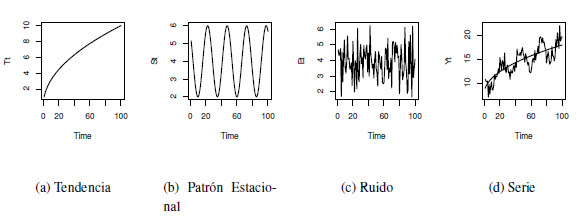
\includegraphics{images/Grafica-tema3-modelo-aditivo} \end{center}

Asumiendo el modelo aditivo, el análisis de series de tiempo consiste en
modelar y estimar \(T_t\) y \(E_t\) y luego extraerlas de \(X_t\) para
obtener \(\hat{\epsilon}_t = X_t - \hat{T}_t - \hat{E}_t\). La serie
\(\hat{\epsilon}_t\) se modela y estima para finalmente reconstruír
\(X_t\), \(\hat{X}_t = \hat{T}_t+\hat{E}_t+\hat{\epsilon}_t\), y poder
realizar el pronóstico
\(\hat{X}_{t+h}=\hat{T}_{t+h}+\hat{E}_{t+h}+\hat{\epsilon}_{t+h}\),
utilizando la información disponible \(X_t,\ldots,X_n\) con
\(h=1,2,\ldots,m\). Sin embargo, puede suceder que la serie
\(\hat{\epsilon}_t\) sea incorrelacionada, es decir,
\(Corr(\hat{\epsilon}_t,\hat{\epsilon}_{t+s}) = 0\), para \(s\neq0\). En
este caso \(\hat{\epsilon}_{t+h}=0\) para todo \(h>0\).

\subsection{El Modelo Multiplicativo de Componentes de Series de
Tiempo}\label{el-modelo-multiplicativo-de-componentes-de-series-de-tiempo}

Dada una serie de tiempo \(X_t,t=1,\ldots,n\), el \emph{Modelo
Multiplicativo de Componentes} consiste en asumir que \(X_t\) se puede
descomponer de una de las siguientes maneras:

\begin{itemize}
\tightlist
\item
  \emph{Puro}:

  \begin{equation}
  X_t = T_t\times E_t\times\epsilon_t
  \label{eq:eq-modelo-multiplicativo-puro}
  \end{equation}
\item
  \emph{Mixto}:

  \begin{equation}
  X_t = T_t\times E_t+\epsilon_t
  \label{eq:eq-modelo-multiplicativo-mixto}
  \end{equation}
\end{itemize}

donde \(T_t\) es la componente de tendencia, \(E_t\) es la componente
estacional y \(\epsilon_t\) es la componente aleatoria o de errores.
Estos modelos son apropiados cuando la magnitud de las fluctuaciones
estacionales de la serie crece y decrece proporcionalmente con los
crecimientos y decrecimientos de la tendencia respectivamente.

\BeginKnitrBlock{definition}
\protect\hypertarget{def:defi-tendencia}{}{\label{def:defi-tendencia} }La
\textbf{tendencia}, se define como una función \(T_t\) de \(t\) que
describe la evolución lenta y a largo plazo del nivel medio de la serie.
La función \(T_t\) depende de parámetros, que deben estimarse.
\EndKnitrBlock{definition}

A continuación presentamos una lista de posibles modelos para la
tendencia \(T_t\):

\begin{itemize}
\tightlist
\item
  Lineal

  \begin{equation}
  T_t=\beta_0+\beta_1t
  \label{eq:eq-modelo-lineal}
  \end{equation}
\item
  Cuadrático

  \begin{equation}
  T_t=\beta_0+\beta_1t+\beta_2t^2
  \label{eq:eq-modelo-cuadratico}
  \end{equation}
\item
  Cúbico

  \begin{equation}
  T_t=\beta_0+\beta_1t+\beta_2t^2+\beta_3t^3
  \label{eq:eq-modelo-cubico}
  \end{equation}
\item
  Exponencial

  \begin{equation}
  T_t=\exp(\beta_0+\beta_1t)
  \label{eq:eq-modelo-exponencial}
  \end{equation}
\item
  Logístico

  \begin{equation}
  T_t=\frac{\beta_2}{1+\beta_1\exp(-\beta_0t)}
  \label{eq:eq-modelo-logistico}
  \end{equation}
\end{itemize}

En la tendencia cuadrática podemos observar:

\begin{itemize}
\tightlist
\item
  Si \(\beta_1,\beta_2>0\), \(T_t\) es monótona creciente.
\item
  Si \(\beta_1,\beta_2<0\), \(T_t\) es monótona decreciente.
\item
  Si \(\beta_1>0\) y \(\beta_2<0\), \(T_t\) es cóncava.
\item
  Si \(\beta_1<0\) y \(\beta_2>0\), \(T_t\) es convexa.
\end{itemize}

\BeginKnitrBlock{definition}
\protect\hypertarget{def:defi-modelo-log-lineal}{}{\label{def:defi-modelo-log-lineal}
}El modelo \textbf{Logarítmico Lineal} o \textbf{Log-Lineal} se define
como

\begin{equation}
\ln X_t = \beta_0+\beta_1t + \epsilon_t
\label{eq:eq-modelo-log-lineal}
\end{equation}
\EndKnitrBlock{definition}

Corresponde a un modelo con tendencia lineal para el logaritmo de
\(X_t\). En \eqref{eq:eq-modelo-log-lineal} al tomar exponencial se tiene
\(X_t = \exp(\beta_0+\beta_1t + \epsilon_t)\), que es similar al modelo
con tendencia exponencial \eqref{eq:eq-modelo-exponencial}. Sin embargo,
son modelos diferentes y se estiman por métodos diferentes.

\section{Estimación de la Tendencia}\label{estimacion-de-la-tendencia}

En esta sección introducimos la estimación de la tendencia mediante
modelos de regresión lineal y no lineal. Son modelos paramétricos.
También introduciremos modelos no paramétricos para estimar la
tendencia, como los suavizadores, los filtros lineales y no lineales y
las medias móviles. Hay otros métodos que no consideraremos en este
curso, por ejemplo, \emph{wavelets}. En ocasiones la expresión
``suavizar una serie'' es equivalente a ``extracción de la tendencia de
una serie'', y ambas equivalen a la estimación de la tendencia.

Para la estimación de los parámetros \(\beta_0,\beta_1,\beta_2\) en los
modelos lineales \eqref{eq:eq-modelo-lineal},
\eqref{eq:eq-modelo-cuadratico}, \eqref{eq:eq-modelo-cubico} y
\eqref{eq:eq-modelo-log-lineal} utilizaremos el método de mínimos
cuadrados clásico (MCC). En este método los parámetros estimados son
aquellos que producen el valor mínimo de la suma de errores cuadrados.
Para los modelos \eqref{eq:eq-modelo-exponencial} y
\eqref{eq:eq-modelo-logistico} se usa el método de mínimos cuadrados no
lineales, que también minimiza la suma de errores cuadrados.

El modelo Log-Lineal \eqref{eq:eq-modelo-log-lineal} es equivalente,
algebráicamente, a \[X_t = \exp(\beta_0 + \beta_1t + \epsilon_t).\] Sin
embargo, este último modelo es no lineal y no coincide con el modelo
exponencial,\eqref{eq:eq-modelo-exponencial},
\(X_t = \exp(\beta_0+\beta_1t)+\epsilon_t\). Es posible estimar por
mínimos cuadrados ordinarios el modelo Log-Lineal y utilizar los
parámetros estimados \(\hat{\beta}_0,\hat{\beta}_1\) como valores
iniciales en la estimación del modelo exponencial por mínimos cuadrados
no lineales. Pero los parámetros estimados en ambos modelos no
necesariamente coinciden.

Aunque la serie tenga una componente estacional \(E_t\),
\(X_t = T_t + E_t + \epsilon_t\), solamente consideramos un modelo de
regresión entre \(X_t\) y \(T_t\), tal que \(X_t = T_t + \eta_t\), donde
\(\eta_t\) es el término de error, de forma que
\(\eta_t=E_t+\epsilon_t\). Por ejemplo,

\begin{enumerate}
\def\labelenumi{\arabic{enumi}.}
\tightlist
\item
  En el caso lineal \(T_t = \beta_0 + \beta_1t\), ajustamos el modelo de
  regresión lineal: \(X_t = \beta_0 + \beta_1t + \eta_t\).
\item
  En el caso cuadrático \(T_t = \beta_0 +\beta_1t+\beta_2t^2\),
  ajustamos el modelo de regresión cuadrático
  \(X_t = \beta_0+\beta_1t+\beta_2t^2 +\eta_t\). Nótese que en este caso
  hay que definir una variable explicativa adicional \(t^2\).
\end{enumerate}

En general, para que datos de series de tiempo sean estacionarias, es
necesario hacer un promedio de productos en el tiempo. Como para datos
de serie de tiempo es importante medir la dependencia entre los valores
de la serie; al menos, debemos ser capaces de estimar las
autocorrelaciones con precisión. Será difícil medir la dependencia de
estos valores si la estructura de dependencia no es regular o si cambia
en el tiempo. De ahí, que para realizar cualquier análisis estadístico
significativo de datos de series de tiempo, será crucial que las
funciones de media y autocovarianza satisfagan las condiciones de
estacionaridad dadas en la Definición 2.4.2. A menudo, este no es el
caso, y en esta sección daremos algunos métodos para lidiar con los
efectos de no-estacionaridad sobre las propiedades estacionarias de las
series a estudiar.

Varios de los ejemplos vistos son claramente no estacionarios. La serie
Johnson \& Johnson en la Figura 2.1 (Tema 2) tiene media que crece
exponencialmente en el tiempo, y el incremento de la magnitud de
fluctuación alrededor de su tendencia causa que la función de
autocovarianza cambie. También, la serie de temperatura global que se
muestra en la Figura 2.2 (Tema 2) contiene evidencia de alguna tendencia
en el tiempo; el calentamiento global es de forma empírica inducida por
el hombre.

Quizás la forma más fácil de trabajar con series no-estacionarias es el
modelo de tendencia estacionaria donde el proceso tiene comportamiento
estacionario alrededor de una tendencia. Podemos escribir este tipo de
modelos como

\begin{equation}
X_t=T_t+Y_t
\label{eq:eq-modelo-tendencia-estacionaria}
\end{equation}

donde \(X_t\) son las observaciones, \(T_t\) denota la tendencia y
\(Y_t\) es un proceso estacionario.

Por lo general, una tendencia fuerte \(T_t\) puede oscurecer el
comportamiento del proceso estacionario \(Y_t\), como veremos en
ejemplos posteriores. De aquí, será una ventaja el que podamos remover
la tendencia como un primer paso para un análisis exploratorio de los
datos. Los pasos envuelven obtener un estimador razonable del componente
de tendencia, llamémoslo \(\hat{T}_t\) y entonces trabajar con el
residual

\begin{equation}
\hat{Y}_t=X_t-\hat{T}_t.
\label{eq:eq-estimacion-componente-tendencia}
\end{equation}

El primer paso en el análisis de cualquier tipo de serie es un gráfico
de los datos.

\begin{itemize}
\item
  Si existe alguna aparente discontinuidad en la serie, tal como un
  cambio súbito en el nivel de la serie, esto puede darnos una idea para
  el análisis de la serie, un primer paso sería dividir la serie en
  segmentos homogéneos.
\item
  Si existen observaciones o datos ``\emph{outliers}'', estos deben ser
  estudiados con cuidado para verificar si existe alguna justificación
  para descartar estas observaciones, como por ejemplo si una
  observación ha sido registrada de algún otro proceso por error.
\item
  La inspección del gráfico también podría sugerir la representación de
  los datos como una realización de un proceso, como el modelo clásico
  de descomposición dado por \eqref{eq:eq-modelo-aditivo}.
\end{itemize}

Si la componente estacional y la componente aleatoria o ruido parecen
incrementarse con el nivel del proceso entonces una transformación
preliminar de los datos es a menudo usada para hacer que los datos
transformados sean compatibles con el modelo \eqref{eq:eq-modelo-aditivo}.
En esta sección discutiremos algunas técnicas para identificar y
eliminar las componentes en @ref(eq:eq-modelo-aditivo\}).

Nuestro objetivo es estimar y extraer las componentes determinísticas
\(T_t\) y \(E_t\) con la esperanza de que el residual o la componente
aleatoria \(\epsilon_t\) llegue a ser un proceso estacionario. Entonces
podremos usar la teoría de tales procesos para hallar un modelo
probabilístico satisfactorio para el proceso \(\epsilon_t\), analizar
sus propiedades y usarlo en conjunto con \(T_t\) y \(E_t\) para hacer
pronósticos y control de \(X_t\).

Los dos enfoques para la eliminación de las componentes de tendencia y
estacional son:

\begin{enumerate}
\def\labelenumi{\arabic{enumi}.}
\tightlist
\item
  Estimación de \(T_t\) y \(E_t\) en el modelo
  \eqref{eq:eq-modelo-aditivo},
\item
  Diferencia de los datos \(X_t\).
\end{enumerate}

Ilustraremos ambos enfoque con varios ejemplos

\subsection{Eliminación de la tendencia en ausencia de
estacionalidad}\label{eliminacion-de-la-tendencia-en-ausencia-de-estacionalidad}

En ausencia de la componente estacional \(E_t\) el modelo
\eqref{eq:eq-modelo-aditivo} llega ser

\begin{equation}
X_t = T_t + \epsilon_t,\quad t=1,\ldots,n
\label{eq:eq-modelo-tendencia}
\end{equation}

donde, sin perdida de generalidad, podemos asumir que
\(E(\epsilon_t)=0\).

\begin{enumerate}
\def\labelenumi{\arabic{enumi}.}
\tightlist
\item
  \textbf{Método T1: Estimación de \(T_t\) por mínimos cuadrados}. En
  este procedimiento intentamos ajustar una familia paramétrica de
  funciones como vimos en la
  sección\textasciitilde{}\ref{seccion-modelo-aditivo}, a los datos
  eligiendo los parámetros que minimicen \(\sum_t(X_t-T_t)^2\).
\end{enumerate}

\BeginKnitrBlock{example}
\protect\hypertarget{exm:ejem-metodo-T1}{}{\label{exm:ejem-metodo-T1}
}Ajustando una función de la forma \eqref{eq:eq-modelo-cuadratico} para la
población de los datos en el gráfico \ref{Grafico-Tema3-poblacion-USA}
para \(1790\leq t\leq1980\) nos da los parámetros estimados
\[\hat{a}_0=2.0978;\quad \hat{a}_1=2.3349\times10^{-3}; \hat{a}_2=6.4984\times10^{-7}.\]
En el gráfico \ref{Grafico-Tema3-poblacion-USA} se puede observar la
curva ajustada y los datos originales. Los valores estimados del proceso
de ruido \(\epsilon_t, 1790\leq t\leq1980\), son los residuales
obtenidos por sustracción de
\(\hat{T}_t=\hat{a}_0+\hat{a}_1t+\hat{a}_2t^2\) de la serie \(X_t\). La
componente de tendencia \(T_t\) nos proporciona un predictor natural de
los valores futuros de \(X_t\). Por ejemplo si deseamos estimar
\(\epsilon_{1990}\) por su valor medio, obtenemos
\[T_{1990} = 2.7588\times10^8\] para la población de EE.UU en 1990. Sin
embargo si los residuales \(\hat{\epsilon}_t\) están altamente
correlacionados podemos ser capaces de usar esos valores para dar una
mejor estimación de \(\epsilon_{1990}\) y por consiguiente de
\(X_{1990}\).
\EndKnitrBlock{example}

\begin{Shaded}
\begin{Highlighting}[]
\NormalTok{uspop=}\KeywordTok{ts}\NormalTok{(}\KeywordTok{scan}\NormalTok{(}\StringTok{"data/USPOP.txt"}\NormalTok{),}\DataTypeTok{frequency=}\DecValTok{1}\OperatorTok{/}\DecValTok{10}\NormalTok{,}\DataTypeTok{start=}\DecValTok{1790}\NormalTok{)}
\NormalTok{pop=}\KeywordTok{window}\NormalTok{(uspop,}\DataTypeTok{start=}\DecValTok{1790}\NormalTok{)}
\NormalTok{x=}\KeywordTok{time}\NormalTok{(pop)}
\NormalTok{reg=}\KeywordTok{lm}\NormalTok{(pop}\OperatorTok{~}\NormalTok{x}\OperatorTok{+}\KeywordTok{I}\NormalTok{(x}\OperatorTok{^}\DecValTok{2}\NormalTok{),}\DataTypeTok{na.action=}\OtherTok{NULL}\NormalTok{)}
\KeywordTok{summary}\NormalTok{(reg)}
\end{Highlighting}
\end{Shaded}

\begin{verbatim}
## 
## Call:
## lm(formula = pop ~ x + I(x^2), na.action = NULL)
## 
## Residuals:
##      Min       1Q   Median       3Q      Max 
## -6947521  -358167   436285  1481410  3391761 
## 
## Coefficients:
##              Estimate Std. Error t value Pr(>|t|)    
## (Intercept)  2.10e+10   6.59e+08    31.9   <2e-16 ***
## x           -2.34e+07   6.98e+05   -33.5   <2e-16 ***
## I(x^2)       6.51e+03   1.85e+02    35.2   <2e-16 ***
## ---
## Signif. codes:  
## 0 '***' 0.001 '**' 0.01 '*' 0.05 '.' 0.1 ' ' 1
## 
## Residual standard error: 2770000 on 18 degrees of freedom
## Multiple R-squared:  0.999,  Adjusted R-squared:  0.999 
## F-statistic: 8.05e+03 on 2 and 18 DF,  p-value: <2e-16
\end{verbatim}

\begin{Shaded}
\begin{Highlighting}[]
\KeywordTok{plot}\NormalTok{(pop,}\DataTypeTok{type=}\StringTok{"o"}\NormalTok{,}\DataTypeTok{ylab=}\StringTok{"Poblacion (millones)"}\NormalTok{)}
\KeywordTok{curve}\NormalTok{(reg}\OperatorTok{$}\NormalTok{coefficient[}\DecValTok{1}\NormalTok{]}\OperatorTok{+}\NormalTok{reg}\OperatorTok{$}\NormalTok{coefficient[}\DecValTok{2}\NormalTok{]}\OperatorTok{*}\NormalTok{x}\OperatorTok{+}\NormalTok{reg}\OperatorTok{$}\NormalTok{coefficient[}\DecValTok{3}\NormalTok{]}\OperatorTok{*}\NormalTok{x}\OperatorTok{^}\DecValTok{2}\NormalTok{,}
      \DataTypeTok{add=}\NormalTok{T,}\DataTypeTok{col=} \StringTok{"red"}\NormalTok{)}
\end{Highlighting}
\end{Shaded}

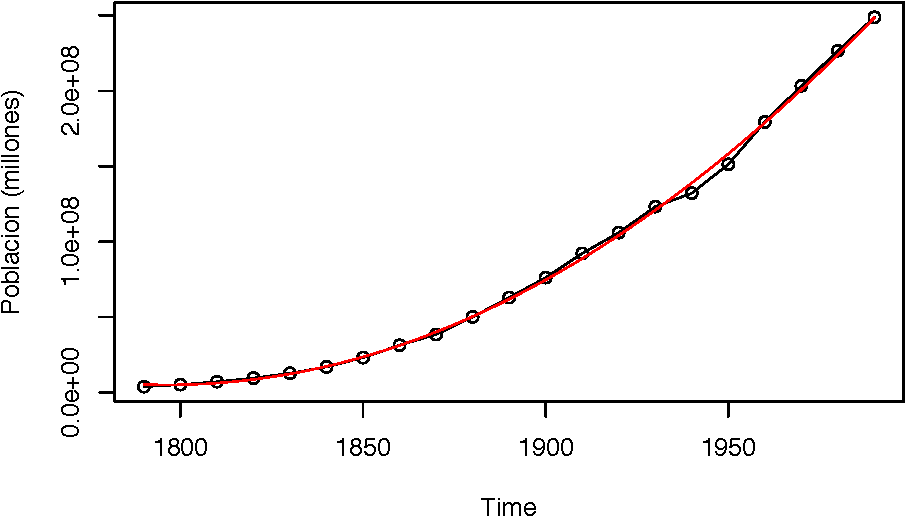
\includegraphics{Serie-de-Tiempo-en-R_files/figure-latex/unnamed-chunk-14-1.pdf}

\begin{enumerate}
\def\labelenumi{\arabic{enumi}.}
\setcounter{enumi}{1}
\tightlist
\item
  \textbf{Método T2: Suavizado por medio de un promedio móvil}. Sea
  \(q\) un entero no negativo y consideremos un promedio móvil de la
  forma

  \begin{equation}
  W_t = \frac{1}{2q+1}\sum_{j=-q}^{q}X_{t+j}
  \label{eq:eq-promedio-movil-orden-q}
  \end{equation}

  de un proceso \(\{X_t\}\) definido por \eqref{eq:eq-modelo-tendencia}.
  Entonces para \(q+1\leq t\leq n-q\),

  \begin{eqnarray}
  W_t &=& \frac{1}{2q+1}\sum_{j=-q}^qT_{t+j}+\frac{1}{2q+1}\sum_{j=-q}^q\epsilon_{t+j}\\ \nonumber
      &\simeq& T_t \label{eq:eq-media-promedio-movil}
  \end{eqnarray}

  suponiendo que \(T_t\) es aproximadamente lineal sobre el intervalo
  \([t-q,t+q]\) y que el promedio del término de error sobre este
  intervalo es cercano a cero.
\end{enumerate}

El promedio móvil entonces nos provee con el estimador

\begin{equation}
      \hat{T}_t = \frac{1}{2q+1}\sum_{j=-q}^qX_{t+j},\quad q+1\leq t\leq n-q.
\label{eq:eq-estimador-promedio-movil}
\end{equation}

Dado que \(X_t\) es no observado para \(t\leq0\) o \(t\geq n\) no
podemos usar (\ref{eq-estimador-promedio-movil}) para \(t\leq q\) o
\(t>n-q\). Una forma de resolver este problema es haciendo \(X_t=X_1\)
para \(t<1\) y \(X_t=X_n\) para \(t>n\). A continuación presentamos un
ejemplo

\BeginKnitrBlock{example}
\protect\hypertarget{exm:ejem-huelgas-USA}{}{\label{exm:ejem-huelgas-USA}
}El gráfico siguiente muestra las huelgas ocurridas en EE.UU, de 1951 a
1980, según la Oficina de Estadísticas Laborales del Departamento de
Trabajo de los EE.UU.

A estos datos le aplicamos un promedio móvil de 5 puntos, la Figura
muestra la serie suavizada y el término de error estimado
\(\hat{\epsilon}_t = X_t - \hat{T}_t\) se muestra en la Figura
\ref{Grafico-tema3-residuales-huelga-USA}. Como era de esperarse ellos
no presentan una tendencia clara.

Las instrucciones en R para el suavizado y los gráficos son los
siguientes:
\EndKnitrBlock{example}

\begin{Shaded}
\begin{Highlighting}[]
\NormalTok{H=}\KeywordTok{read.table}\NormalTok{(}\StringTok{"data/Huelgas.txt"}\NormalTok{)}
\KeywordTok{plot}\NormalTok{(H,}\DataTypeTok{xlab=}\StringTok{"anos"}\NormalTok{,}\DataTypeTok{ylab=}\StringTok{"Huelgas"}\NormalTok{,}\DataTypeTok{type=}\StringTok{'b'}\NormalTok{)}
\end{Highlighting}
\end{Shaded}

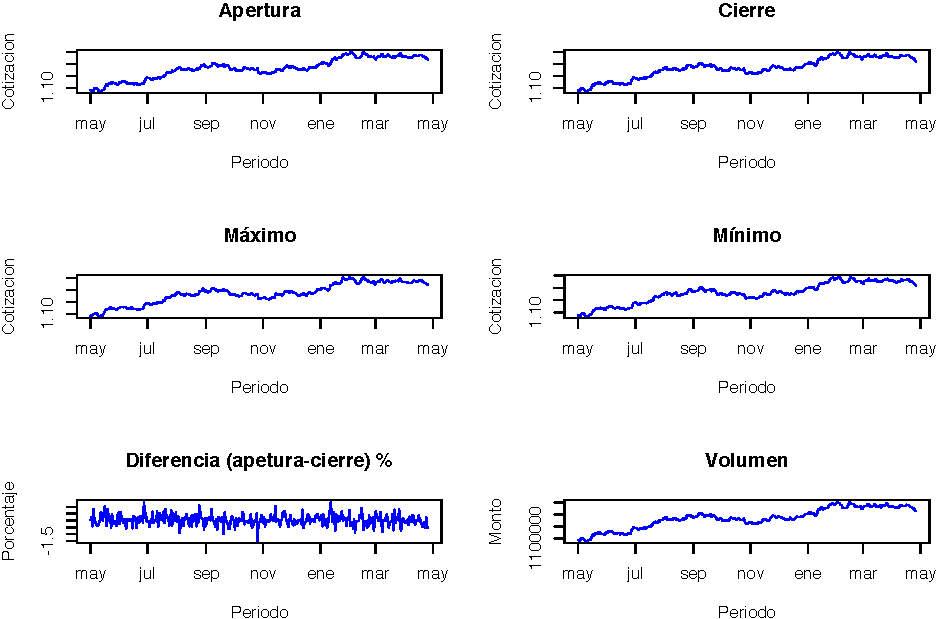
\includegraphics{Serie-de-Tiempo-en-R_files/figure-latex/unnamed-chunk-15-1.pdf}

\begin{Shaded}
\begin{Highlighting}[]
\NormalTok{W=}\KeywordTok{filter}\NormalTok{(H[,}\DecValTok{2}\NormalTok{],}\DataTypeTok{sides=}\DecValTok{2}\NormalTok{,}\KeywordTok{rep}\NormalTok{(}\DecValTok{1}\OperatorTok{/}\DecValTok{5}\NormalTok{,}\DecValTok{5}\NormalTok{))}
\KeywordTok{plot}\NormalTok{(H[,}\DecValTok{1}\NormalTok{],W,}\DataTypeTok{xlab=}\StringTok{"anos"}\NormalTok{,}\DataTypeTok{ylab=}\StringTok{"Huelgas"}\NormalTok{,}\DataTypeTok{type=}\StringTok{'b'}\NormalTok{)}
\end{Highlighting}
\end{Shaded}

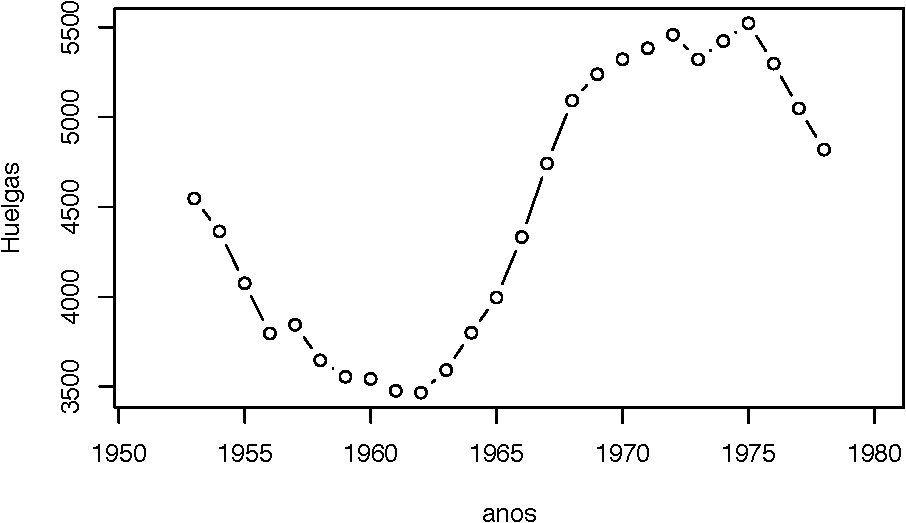
\includegraphics{Serie-de-Tiempo-en-R_files/figure-latex/unnamed-chunk-15-2.pdf}

\begin{Shaded}
\begin{Highlighting}[]
\NormalTok{y=H[,}\DecValTok{2}\NormalTok{]}\OperatorTok{-}\NormalTok{W}
\KeywordTok{plot}\NormalTok{(H[,}\DecValTok{1}\NormalTok{],y,}\DataTypeTok{xlab=}\StringTok{"anos"}\NormalTok{,}\DataTypeTok{ylab=}\StringTok{"Residuales"}\NormalTok{,}\DataTypeTok{type=}\StringTok{'b'}\NormalTok{)}
\end{Highlighting}
\end{Shaded}

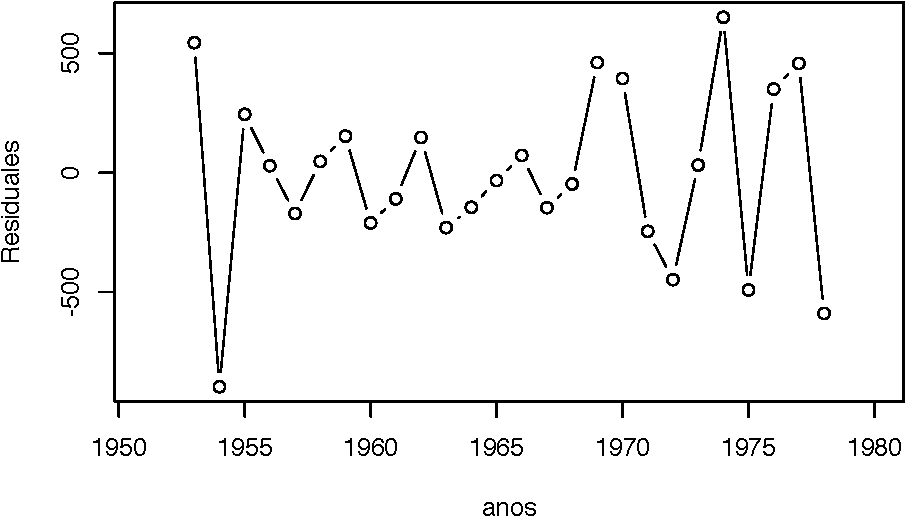
\includegraphics{Serie-de-Tiempo-en-R_files/figure-latex/unnamed-chunk-15-3.pdf}

Para cada valor fijo \(a\in[0,1]\), el promedio móvil de un lado
\(\hat{T}_t, t=1,\ldots,n\), definido por la recursión

\begin{equation}
  \hat{T}_t = aX_t+(1-a)\hat{T}_t,\quad t=2,\ldots,n
 \label{eq:eq-promedio-movil-1-lado-peso}
\end{equation}

y

\[\hat{T}_1=X_1,\] se puede calcular usando la opción \emph{sides=1} en
la función \emph{filter} de R.

Es usual pensar como aplicación de la ecuación
\eqref{eq:eq-promedio-movil-1-lado-peso} como un suavizado exponencial,
dado que se sigue de la recursión que para
\(t\leq2, \hat{T}_t=\sum_{j=0}^{t-2}a(1-a)^jX_{t-j}+(1-a)^{t-1}X_1\), es
un promedio móvil con peso de \(X_t,X_{t-1},\ldots\), con pesos
decreciendo exponencialmente (excepto para el último término).

Es útil pensar en \(\{\hat{T}_t\}\) en (\emph{filter}) como un proceso
obtenido de \(\{X_t\}\) por aplicación de un operador lineal o filtro
lineal \(\hat{T}_t=\sum_{j=-\infty}^{\infty}a_jX_{t+j}\) con pesos
\(a_j=(2q+1)^{-1},-q\leq j\leq q\), y \(a_j=0,|j|>q\). Este filtro
particular es un filtro de ``paso-bajo'' ya que toma los datos
\(\{X_t\}\) y remueve la componente de rápida fluctuación (o de alta
frecuencia) \(\{\hat{\epsilon}_t\}\), para dejar el término de la
tendencia estimada de lenta variación \(\{\hat{T}_t\}\).

\begin{itemize}
\tightlist
\item
  \textbf{Método T3: Diferenciación para generar datos estacionarios}.
  En lugar de intentar remover el ruido por suavizado como en el Método
  T2, ahora intentaremos eliminar la tendencia por diferenciación.
  Definamos primero el operador diferencia \(\nabla\) por

  \begin{equation}
    \nabla x_t = x_t-x_{t-1}=(1-B)x_t,
  \label{eq:eq-operador-diferencia}
  \end{equation}

  donde \(B\) es el operador de desplazamiento hacia atrás
  (\emph{backward shift operator} en inglés),

  \begin{equation}
    Bx_t=x_{t-1}.
  \label{eq:eq-backward-shift-operator}
  \end{equation}

  Las potencias de los operadores \(B\) y \(\nabla\) se definen de
  manera obvia, esto es, \(B^j(x_t)=x_{t-j}\) y
  \(\nabla^j(x_t)=\nabla(\nabla^{j-1}(x_t)),j\geq1\) con
  \(\nabla^0(x_t)=x_t\). Los polinomios en \(B\) y \(\nabla\) se
  manipulan de la misma manera que las funciones polinómicas de
  variables reales. Por ejemplo

  \begin{eqnarray*}
    \nabla^2x_t &=& \nabla(\nabla x_t) = (1-B)(1-B)x_t = (1-2B+B^2)x_t \\
            &=& x_t-2x_{t-1}+x_{t-2}.
  \end{eqnarray*}

  Si el operador \(\nabla\) se aplica a una función con tendencia lineal
  \(T_t=at+b\), entonces obtenemos la función constante
  \(\nabla T_t=a\). De la misma manera cada tendencia polinomial de
  grado \(k\) se puede reducir a una constante por aplicación del
  operador \(\nabla^k\).
\end{itemize}

Iniciando entonces con el modelo \(X_t=T_t+\epsilon_t\), donde
\(T_t=\sum_{j=0}^ka_jt^j\) y \(\epsilon_t\) es estacionario con media
cero, obtenemos

\[\nabla^kX_t = k!a_k+\nabla^k\epsilon_t,\] un proceso estacionario con
media \(k!a_k\). Esta consideración sugiere la posibilidad, dada una
sucesión \(\{X_t\}\) de datos, de aplicar el operador \(\nabla\)
repetidamente hasta conseguir una sucesión \(\{\nabla^kX_t\}\) la cual
puede ser apropiadamente modelada como una realización de un proceso
estacionario. Se encuentra a menudo en la práctica que el orden \(k\) de
diferenciación es bastante pequeño, frecuentemente uno o
dos.\footnote{Esto depende del hecho de que muchas funciones pueden ser aproximadas bastante bien, en un intervalo de longitud finita, por un polinomio de grado razonablemente bajo.}

Aplicando esta técnica al ejemplo de los 20 datos de población de los
EE.UU, hallamos que dos operaciones de diferenciación son suficientes
para producir una serie sin aparente tendencia. Los datos diferenciados
se muestran en la Figura \ref{Grafico-Tema3-diferencias-poblacion-USA}.
Note que la magnitud de las fluctuaciones en \(\nabla^2X_n\) se
incrementa con el valor de \(n\). Este efecto se puede suprimir tomando
primero logaritmo natural, \(y_n=\ln X_n\) y entonces aplicando el
operador \(\nabla^2\) a la serie \(\{y_n\}\).

Las instrucciones en R son las siguientes

\begin{Shaded}
\begin{Highlighting}[]
\NormalTok{Dx=}\KeywordTok{diff}\NormalTok{(uspop,}\DataTypeTok{difference=}\DecValTok{2}\NormalTok{)}
\end{Highlighting}
\end{Shaded}

\section{Eliminación de la tendencia y la
estacionalidad}\label{eliminacion-de-la-tendencia-y-la-estacionalidad}

Los métodos descritos para remover la tendencia pueden ser adaptados de
manera natural para eliminar tanto la tendencia como la estacionalidad
en el modelo general

\begin{equation}
X_t = T_t + E_t + \epsilon_t
\end{equation}

donde \(E\epsilon_t=0, E_{t+d}=E_t\) y \(\sum_{j=1}^dE_t=0\).
Ilustraremos estos métodos con referencia al siguiente ejemplo de
accidentes. En la Tabla\textasciitilde{}\ref{tabla-accidentes-USA} se
muestran los datos, y en la
Figura\textasciitilde{}\ref{Grafico-tema3-accidentes-USA} podemos
observar que en los mismos se ve claramente una componente estacional
con periodo \(d=12\).

\begin{longtable}[]{@{}ccccccc@{}}
\toprule
mes/año & 1973 & 1974 & 1975 & 1976 & 1977 & 1978\tabularnewline
\midrule
\endhead
Ene & 9007 & 7750 & 8162 & 7717 & 7792 & 7836\tabularnewline
Feb & 8106 & 6981 & 7306 & 7461 & 6957 & 6892\tabularnewline
Mar & 8928 & 8038 & 8124 & 7776 & 7726 & 7791\tabularnewline
Abr & 9137 & 8422 & 7870 & 7925 & 8106 & 8129\tabularnewline
May & 10017 & 8714 & 9387 & 8634 & 8890 & 9115\tabularnewline
Jun & 10826 & 9512 & 9556 & 8945 & 9299 & 9434\tabularnewline
Jul & 11317 & 10120 & 10093 & 10078 & 10625 & 10484\tabularnewline
Ago & 10744 & 9823 & 9620 & 9179 & 9302 & 9827\tabularnewline
Sep & 9713 & 8743 & 8285 & 8037 & 8314 & 9110\tabularnewline
Oct & 9938 & 9129 & 8433 & 8488 & 8850 & 9070\tabularnewline
Nov & 9161 & 8710 & 8160 & 7874 & 8265 & 8633\tabularnewline
Dic & 8927 & 8680 & 8034 & 8647 & 8796 & 9240\tabularnewline
\bottomrule
\end{longtable}

Accidentes mortales mensuales en EE.UU., años 1973-1978.

Será conveniente para el primer método indexar los datos por año y mes.
Entonces \(X_{j,k}, j=1,\ldots,6, k=1,\ldots,12\) denotará el número de
muertes accidentales reportados para el \(k\)-ésimo mes del \(j\)-ésimo
año, (1972+j). En otras palabras, definimos
\[X_{j,k}=X_{k+12(j-1)}, j=1,\ldots,6, k=1,\ldots,12.\]

\begin{itemize}
\tightlist
\item
  \textbf{Método E1: Método de la tendencia pequeña}. Si la tendencia es
  pequeña (como en los datos de accidentes) no es irrazonable suponer
  que el término de la tendencia es constante, digamos \(T_j\) para el
  año \(j\). Dado que \(\sum_{k=1}^{12}E_k=0\), nos lleva al estimador
  insesgado natural

  \begin{equation}
  \hat{T}_j = \frac{1}{12}\sum_{k=1}^{12}X_{j,k},
  \label{eq:eq-estimador-Tj-accidentes}
  \end{equation}

  mientras que para \(E_k, k=1,\ldots,12\) tenemos el estimador

  \begin{equation}
  \hat{E}_t = \frac{1}{6}\sum_{j=1}^6(X_{j,k}-\hat{T}_j),
  \label{eq:eq-estimador-Et-accidentes}
  \end{equation}

  el cual automáticamente satisface el requisito de que
  \(\sum_{k=1}^{12}\hat{E}_k=0\). El término de error estimado para el
  mes \(k\) del año \(j\) es por supuesto

  \begin{equation}
  \hat{\epsilon}_{j,k} = X_{j,k}-\hat{T}_j-\hat{E}_k, \quad j=1,\ldots,6,k1,\ldots,12.
  \label{eq:eq-estimador-epsilon-t-accidentes}
  \end{equation}

  La generalización de (\ref{eq-estimador-Tj-accidentes}) a
  (\ref{eq-estimador-epsilon-t-accidentes}) para datos con
  estacionalidad con un periodo distinto de 12 es bastante claro.
\end{itemize}

Las Figuras \ref{Grafico-tema3-accidentes-sin-tendencia},
\ref{Grafico-tema3-accidentes-estacional} y
\ref{Grafico-tema3-accidentes-sin-tendencia-estacional} muestran
respectivamente las observaciones con la tendencia removida
\(X_{j,k}-\hat{T}_j\), la componente estacional estimada \(\hat{E}_t\) y
las observaciones con la tendencia y la estacionalidad removida
\(\hat{\epsilon}_{j,k}=X_{j,k}-\hat{T}_j-\hat{E}_k\). En la última no se
observa una aparente tendencia o estacionalidad.

\begin{itemize}
\tightlist
\item
  \textbf{Método E2: Estimación por promedio móvil}. La siguiente
  técnica es preferible al Método S1 ya que no se basa en la suposición
  de que \(T_t\) es casi constante sobre cada ciclo estacional.
\end{itemize}

Suponga que tenemos las observaciones \(\{x_1,\ldots,x_n\}\). Se estima
primero la tendencia aplicando un filtro de promedio móvil especialmente
elegido para eliminar la componente estacional y para amortiguar el
ruido. Si el periodo \(d\) es par, digamos \(d=2q\), entonces usamos

\begin{equation}
\hat{T}_t = (0.5x_{t-q} + x_{t-q+1} + \cdots + x_{t+q-1} + 0.5x_{t+q})/d, q<t\leq n-q.
\label{eq:eq-filtro-especial-metodo-S2}
\end{equation}

Si el periodo es impar, digamos \(d=2q+1\), entonces usamos el promedio
móvil simple (\ref{eq-estimador-promedio-movil}). La
Figura\textasciitilde{}\ref{Grafico-tema3-accidentes-promedio-movil}
muestra la tendencia estimada \(\hat{T}_t\) para los datos de accidentes
mortales obtenido de (\ref{eq-filtro-especial-metodo-S2}). También
muestra la tendencia constante a trozos obtenida por el Método S1.

El segundo paso, es estimar la componente estacional. Para cada
\(k=1,\ldots,d\), calculamos el promedio \(w_k\) de las desviaciones
\(\{(X_{k+jd}-\hat{T}_{k+jd}):q<k+jd\leq n-q\}\). Dado que este promedio
de desviaciones no necesariamente suma cero, estimamos la componente
estacional \(E_k\) como

\begin{equation}
\hat{E}_k = w_k -\frac{1}{d}\sum_{i=1}^dw_i,\quad i=1,\ldots,d,
\label{eq:eq-estimador-Et-metodo-S2}
\end{equation}

y \(\hat{E}_k=\hat{E}_{k-d},k>d\).

Los datos sin la componente estacional se definen entonces como la serie
original con la componente estacional removida, es decir,

\begin{equation}
d_t = X_t-\hat{E}_t,\quad t=1,\ldots,n.
\label{eq:eq-serie-destacionalizada}
\end{equation}

Finalmente, reestimamos la tendencia de \(\{d_t\}\) aplicando un filtro
de promedio móvil como se describió para los datos no estacionales o
fijando un polinomio a la serie \(\{d_t\}\). El término del ruido
estimado llega a ser entonces

\[\hat{\epsilon}_t = X_t - \hat{E}_t - \hat{E}_t, \quad t=1,\ldots,n.\]
Los resultados de aplicar los Métodos S1 y S2 a los datos de accidentes
mortales son casi iguales, dado que en este caso la constante a trozos y
el promedio móvil de \(T_t\) están razonablemente cercanos.

Una comparación de los valores estimados de \(E_k, k=1,\ldots,12\),
obtenido con ambos métodos se muestra en la
Tabla\textasciitilde{}\ref{Tabla-tema3-componentes-estacionales-estimadas}

\begin{longtable}[]{@{}ccccccccccccr@{}}
\toprule
k & 1 & 2 & 3 & 4 & 5 & 6 & 7 & 8 & 9 & 10 & 11 & 12\tabularnewline
\midrule
\endhead
\(\hat{E}_t(S1)\) & -7434 & -1504 & -724 & -523 & 338 & 808 & 1665 & 961
& -87 & 197 & -321 & -67\tabularnewline
\(\hat{E}_t(S2)\) & -804 & -1522 & -737 & -526 & 343 & 746 & 1680 & 987
& -109 & 258 & -259 & -57\tabularnewline
\bottomrule
\end{longtable}

Componentes estacional estimadas para los datos de accidentes mortales

\begin{itemize}
\tightlist
\item
  \textbf{Método E3: Diferenciación a paso \(\mathbf{d}\)}. La técnica
  de diferenciación la cual aplicamos antes a datos no estacionales se
  pueden adaptar para lidiar con el caso estacional de periodo \(d\)
  introduciendo el operador de diferencia de paso \(d\) \(\nabla_d\)
  definido por

  \begin{equation}
  \nabla_dX_t = X_t-X_{t-d} = (1-B^d)X_t.
  \label{eq:eq-operador-diferencia-paso-d}
  \end{equation}

  Este operador no debe confundirse con el operador
  \(\nabla^d = (1-B)^d\) definido por (\ref{eq-operador-diferencia}).
\end{itemize}

Aplicando el operador \(\nabla_d\) al modelo
\[X_t = T_t + E_t + \epsilon_t,\] donde \(\{E_t\}\) tiene periodo \(d\),
obtenemos \[\nabla_dX_t = T_t-T_{t-d} + \epsilon_t-\epsilon_{t-d},\] lo
cual nos da una descomposición de la diferencia \(\nabla_dX_t\) en una
componente de tendencia \((T_t-T_{t-d})\) y un término de ruido
\((\epsilon_t-\epsilon_{t-d})\). La tendencia \((T_t-T_{t-d})\) se puede
eliminar usando los métodos ya descritos, por ejemplo, aplicando alguna
potencia del operador \(\nabla\). La
Figura\textasciitilde{}\ref{Grafico-tema3-diferencia-paso-12} muestra el
resultado de aplicar el operador \(\nabla_{12}\) a los datos de
accidentes mortales. La componente estacional evidente en la
Figura\textasciitilde{}\ref{Grafico-tema3-accidentes-USA} está ausente
en la Figura de \(\nabla_{12}X_t,13\leq t\leq72\). Sin embargo todavía
parece haber una tendencia decreciente. Si ahora aplicamos el operador
\(\nabla\) a \(\nabla_{12}X_t\) y graficamos las diferencias
\(\nabla\nabla_{12}X_t,t=14,\ldots,72\) obtenemos el gráfico mostrado en
la
Figura\textasciitilde{}\ref{Grafico-tema3-diferencia-diferencia-paso-12},
los cuales no tienen una aparente tendencia o componente estacional.

\cleardoublepage 

\appendix \addcontentsline{toc}{chapter}{\appendixname}


\bibliography{book.bib,packages.bib}

\backmatter
\printindex

\end{document}
